\chapter{Convolutional Neural Networks}\label{ch:cnn}
Convolutional Neural Network (CNN) is a class of Artificial Neural Networks\footnote{A computational model inspired by
animal brain.}, which allows for efficient training on high dimensional data.
This is especially useful in the field of \textit{computer vision}\footnote{A scientific field dealing with extraction
of high level understanding from imagery using computers.} as image data is fundamentally high dimensional.

This thesis is dealing with a subset of computer vision called \textit{face recognition}\ref{ch:face-rec} in which CNNs
achieve state-of-the-art results.
For this reason, this chapter is present in the text.

Typical architecture of CNNs contains many layers.
Because of that, these models belong to the class of machine learning methods called
\textit{deep learning}\footnote{A set of machine learning models with \textit{credit assignment path (CAP)} higher than 2.
The CAP is the chain of transformations from input to output.}
In the following section~\ref{sec:layer-types} I will deal with layer types used in CNNs.

\begin{figure}[H]
    \centering
    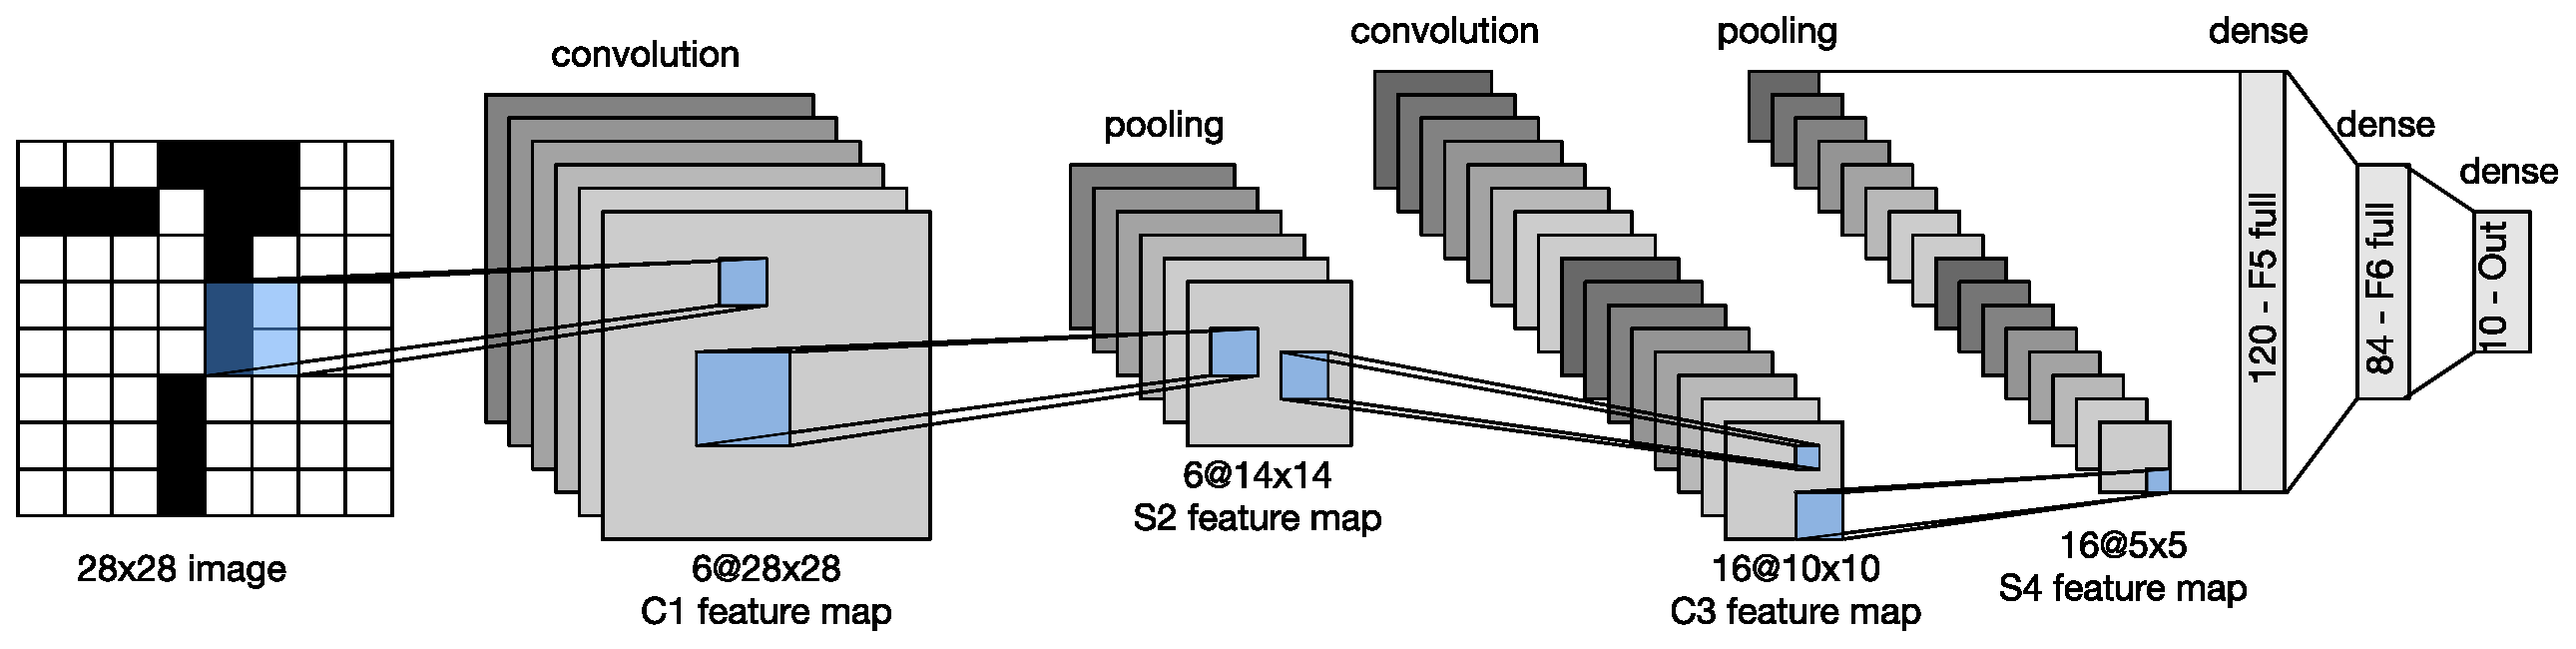
\includegraphics[width=\columnwidth]{images/cnn/lenet.eps}
    \caption{Example of CNN model (LeNet 5)~\cite{LeNet5}}
    \label{fig:cnn}
\end{figure}

\section{Layer Types}\label{sec:layer-types}
The image~\ref{fig:cnn} is an illustration of one of the oldest CNN models, called \textit{LenNet 5}, which was used for
handwritten character recognition.
There are three layer types in the architecture: \textit{dense}~\ref{subsec:dense},
\textit{convolutional}~\ref{subsec:convolutional} and \textit{pooling}~\ref{subsec:pooling} layer.
Modern CNNs also usually contain \textit{locally connected layer}~\ref{subsec:lclayer} and
\textit{ReLU}~\ref{subsec:relu} layer.

\subsection{Dense/Fully Connected}\label{subsec:dense}
Dense layer is the simplest type of layer present in CNN models.
Its output is determined simply by multiplication of its \textit{inputs} (x) with \textit{weight matrix}
(denoted V in~\ref{eq:dense}, also called kernel) and addition of \textit{bias} (u).

\begin{equation}
    \label{eq:dense}
    h[i, j] = u[i,j] + \sum_{a,b} V[i,j,a,b] \cdot x[i+a,j+b]
\end{equation}

To demonstrate the amount of parameters needed, let's imagine that we want to feed a greyscale image which is 256 pixel
high and wide to a dense layer.
First we flatten the image which results in a vector with $256\cdot256 = 65536$ dimensions.
Even if we do aggressive reduction to 1000 hidden dimensions, we end up with approximately 65 million parameters.
This makes dense layer impractical when dealing with imagery.
For this reason a convolutional layer~\ref{subsec:convolutional} is usually used as the input layer of computer
vision models.

\subsection{Convolutional}\label{subsec:convolutional}
As I hinted in the previous section, the main advantage of CNNs~\cite{ConvLayer} is the low amount of parameters needed.
In the convolutional layer this feat was achieved by application of two principles:
\textit{invariance}~\ref{subsec:invariance} and \textit{locality}~\ref{subsec:locality}.

\subsubsection{Invariance Principle}\label{subsec:invariance}
The core of the invariance principle is a reuse of weights.
This is achieved by application of weights on one part of the image, shifting the weights by a predetermined set
of pixels (called a stride) and then applying the weights again.
Let us examine the equation~\ref{eq:denseinv} too see how the original equation~\ref{eq:dense} changes.

\begin{equation}
    \label{eq:denseinv}
    h[i, j] = u + \sum_{a,b} V[a,b] \cdot x[i+a,j+b]
\end{equation}

As is to be expected, bias \textit{u} and the weight matrix \textit{V} are no longer dependent upon the image
coordinates \textit{(i, j)}.
As an example we can think of an airplane detection algorithm whose goal is to find whether there is an airplane
present in any part of the scene.
The core principle used during the algorithm design would be sliding one set of weights (kernel) describing the
airplane over the image.
The algorithm would then classify the scene with high impulse response as containing an airplane.
This intuitively makes a lot of sense.

This type of invariance is called \textit{translational invariance}.

\subsubsection{Locality Principle}\label{subsec:locality}
Another principle used in CNNs is called \textit{locality principle}.
This principle suggests, that we do not need to look far away from \textit{(i,j)} to gain valuable information about
what is going on in that particular location.
This is achieved, mathematically speaking, by limiting \textit{a} and \textit{b} to a range $\Delta$.

\begin{equation}
    \label{eq:denseinvloc}
    h[i, j] = u + \sum_{a=-\Delta}^{\Delta} \sum_{b=-\Delta}^{\Delta} V[a,b] \cdot x[i+a,j+b]
\end{equation}

Equation~\ref{eq:denseinvloc} is the final form describing the convolution layer.

\subsection{Pooling}\label{subsec:pooling}
The main objective of pooling is to decrease the spatial dimension of the inner representation of the data.
During classification (the most common application of CNNs) we are not interested in the location of the classified
object within the image.
The only information that interests us is whether the object is present in the scene or not.
With this information in mind, pooling~\cite{PoolingLayer} was invented.

The pooling layer is similar to the convolutional layer in a sense that both are "looking" only at a part of the input
at once.
This point of view (window) is then shifted as I described in the section~\ref{subsec:invariance}.
What makes the pooling layer different from the convolutional one is that there is no kernel present in the operation.
The only thing pooling does is that it selects/computes the most representative value from the window.
There are two common pooling types: \textit{max pooling} and \textit{average pooling}.
The first type selects the maximum value and the second one computes the average.

Stacking pooling layer on top of convolutional layer is a powerful combination as pooling makes the output of CNNs
more robust to local translations\cite{DeepFace}.

\subsection{Locally Connected}\label{subsec:lclayer}
Locally connected layer is similar to convolutional layer but the difference is that every location in the feature map
learns different set of filters.
This layer type is for example used by the DeepFace system~\ref{subsec:deepface}.

\subsection{ReLU}\label{subsec:relu}

\begin{wrapfigure}{r}{7cm}
    \label{fig:relu}
    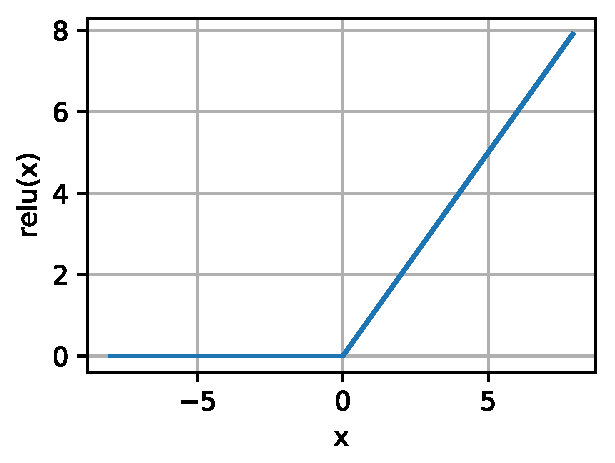
\includegraphics[width=7cm]{images/cnn/relu.eps}
    \caption{Illustration of ReLU activation function~\cite{ReLU}}
\end{wrapfigure}

Rectified linear unit (ReLU) layer applies the activation function\footnote{The activation
function of a node defines the output of that node given an input or set of inputs.}~\ref{eq:relu} to the output of
the preceding layer.
In CNNs the layer is usually positioned at the output of convolutional layer~\ref{subsec:convolutional}.

\begin{equation}
    \label{eq:relu}
    ReLU(x) = max(0,x)
\end{equation}

The advantage of ReLU is its efficacy during the training and the reduced likelihood of a vanishing
gradient\footnote{\label{foot:vangrad}A situation where a deep neural network is unable to propagate useful gradient
information from the output end of the model back to the layers near the input end of the model.}.

\section{Padding}\label{sec:padding}
To avoid loss of information at the edges of the image we usually use a method called \textit{padding}.
This technique increases the image dimension by pixel addition around the original image.
There are few padding variants which are differentiated by the value of the new pixels.
The most common ones are \textit{zero padding} and \textit{reflective padding}.
The first mentioned type, as the name implies, sets the new pixels to zero.
The second one is more sophisticated and consists in mirroring of the neighboring pixels.

\section{Modern Models}\label{sec:models}
This section contains an overview of selected modern models used extensively in facial recognition tasks.

\subsection{InceptionNet}\label{subsec:inceptionnet}
InceptionNets are a class of models in which there are multiple kernel sizes operating at the same level.
This is desirable because the right kernel size is dependent on how globally the information is distributed.
A large kernel is preferred when the information is distributed globally and, vice versa.

\begin{figure}[H]
    \centering
    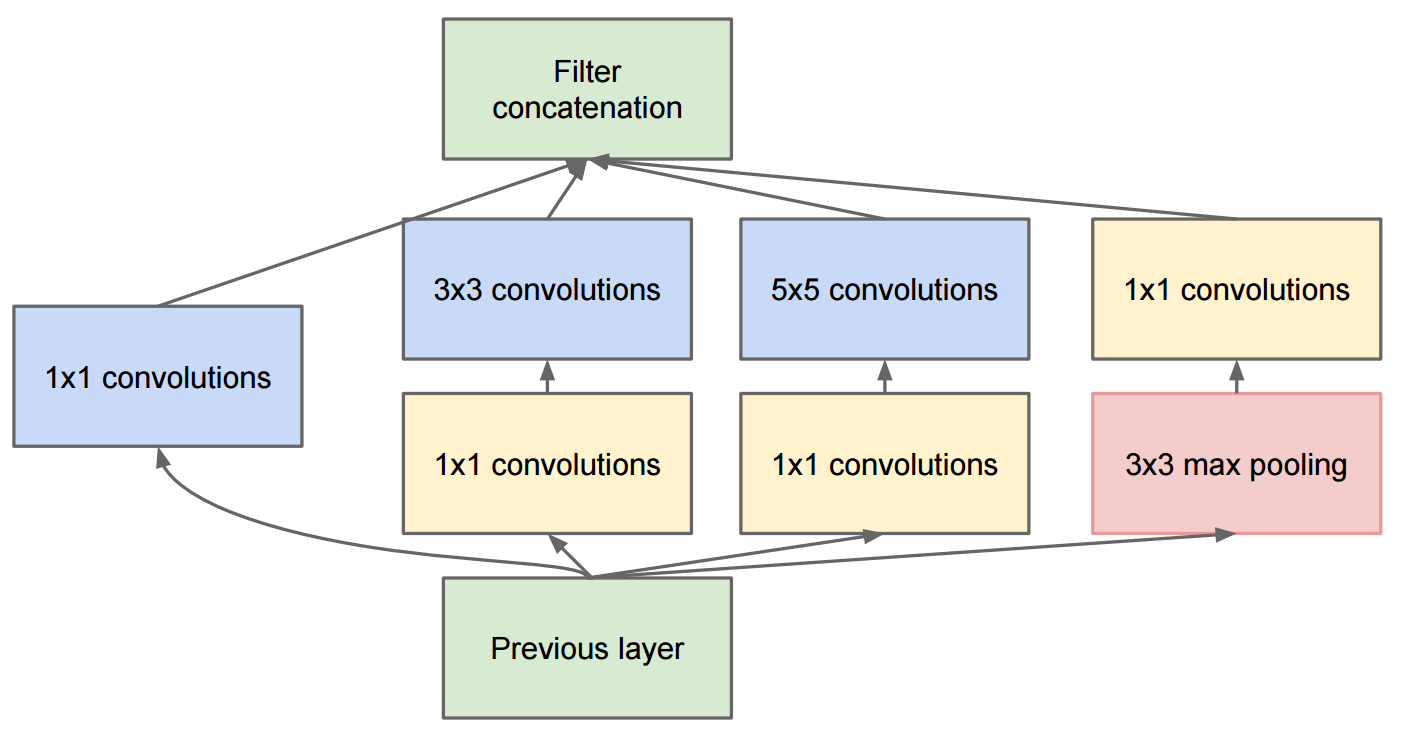
\includegraphics[width=0.9\columnwidth]{images/face-recognition/inceptionnet.png}
    \caption{InceptionNet block~\cite{GoingDeeper}}
    \label{fig:InceptionNet}
\end{figure}

The inception of the inception block (figure~~\ref{fig:InceptionNet}) took place in 2014 in the paper~\cite{GoingDeeper}
published by Google Inc.
Models using inception blocks kept on improving and at the time of writing, there is the fourth version in use.

\subsection{ResNet}\label{subsec:resnet}
A residual neural network (ResNet)~\cite{ResNet} is an Artificial Neural Network (ANN) which allows for the training of
very deep neural networks containing tens of layers.
Training of ANNs this deep had been practically impossible before the invention of ResNet due to the problem of
\textit{vanishing gradient} and \textit{degradation problem}.
The first problem is exposed as a lack of convergence and the second one as a high training error.

Both of these problems have been avoided by implementation of \textit{skip connections} which are illustrated in the
figure~\ref{fig:ResNet}.

\begin{figure}[H]
    \centering
    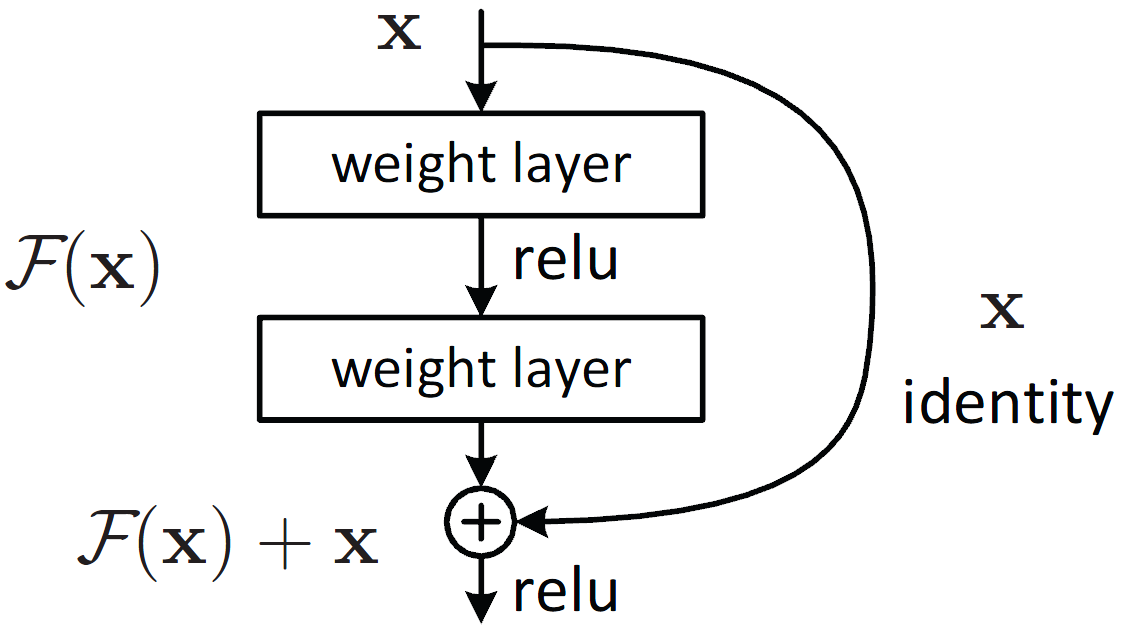
\includegraphics[width=0.9\columnwidth]{images/face-recognition/resnet.png}
    \caption{Residual learning~\cite{ResNet}}
    \label{fig:ResNet}
\end{figure}

The skip connections are implemented as elementwise addition and they let the in-between layers fit a residual mapping.

ResNets are widely used in the field of facial recognition as well as in the field of computer vision as a whole.

In the experimental part, I use 18-layer version called ResNet-18 (see section~\ref{ch:implementation}).

\subsubsection{Architecture of ResNet-18}\label{subsubsec:resnet18}
In the architecture, there are 17 convolutional layers and 1 dense layer.
As is usual, the dense layer is placed at the output.
Each of these layers is followed by batch normalization.
The dimensionality of the first layer's feature map is reduced by max pooling.
ReLu is used extensively within the whole architecture.

\subsection{DenseNet}\label{subsec:densenet}
DenseNet~\cite{DenseNet} is a type of CNN~\ref{ch:cnn} which was introduced in 2017.
The difference from regular CNNs is that every layer is connected to all the subsequent layers.
Traditional CNN with \textit{L} layers has exactly \textit{L} connections.
On the other hand DenseNet with the same amount of layers contains $\frac{L\left( L+1 \right)}{2}$ connections.
The block of layers is illustrated in the figure~\ref{fig:DenseNet}.

\begin{figure}[H]
    \centering
    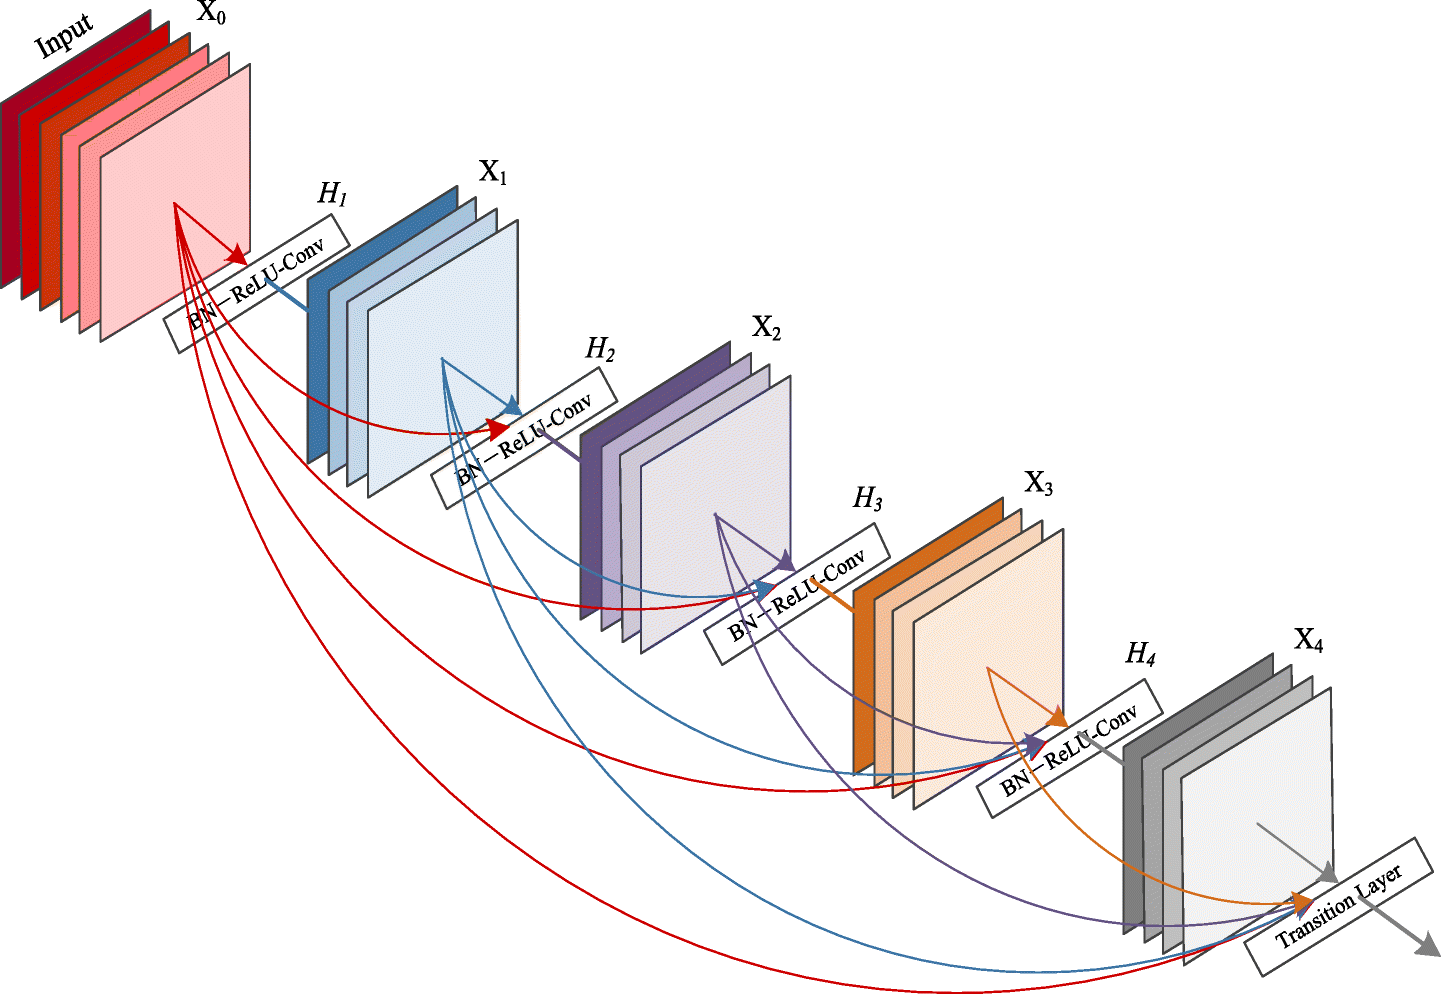
\includegraphics[width=0.9\columnwidth]{images/face-recognition/densenet.png}
    \caption{A 5-layer dense block~\cite{DenseNet}}
    \label{fig:DenseNet}
\end{figure}

DenseNets implement the connections with preceding layers differently than ResNets.
While ResNets use elementwise addition, DenseNets concatenate the feature maps.
The big size of the feature map is not an issue because it is fed as an input into a convolutional layer,
and consequently, the training does not require training more parameters.

DenseNets have several compelling advantages~\cite{DenseNet}.
They alleviate the vanishing-gradient problem, strengthen feature propagation, encourage feature reuse, and
substantially reduce the number of parameters.